



% \begin{figure}[t]
%     \centering
%     \includegraphics[width=0.63\linewidth]{figures/median-dist-vs-reported-replacement-small.pdf}
%     
\includegraphics[width=0.33\linewidth]{figures/cis_iqm_vs_median_all_algos.pdf}
%     \caption{\textbf{Left}. \textbf{Distribution of median normalized scores} computed using 100,000 different sets of $N$ runs subsampled uniformly with replacement from 100 runs.  For a given algorithm, the sampling distribution shows the variation in the median scores when re-estimated using a different set of runs. The reported \emph{point estimates} of median, as shown by dashed lines, do not provide any information about the variability in median scores and severely overestimate or underestimate the expected median. We use the same number of runs as reported by publications: $N=5$ runs for \der, \otr\ and \drq, $N=10$ runs for \spr\ and $N=20$ runs for \curl. \textbf{Right}. \textbf{95\% CIs} for median and IQM scores~(\figref{fig:aggregate_metrics}) for varying $N$. There is a substantial uncertainty in median scores even with 50 runs. IQM has much smaller CIs than median. While improvement from SPR over DER with $5$ to $25$ runs is not statistically significant, claiming ``no improvement'' would also be misleading as evaluating more runs indeed shows that the improvement is significant.}
%     \label{fig:variability_in_median}
%     \vspace{-0.45cm}
% \end{figure}


% \begin{figure}[t]
%     \begin{minipage}[t]{0.59\linewidth}
%     \centering
%         \vspace{1pt}
%         \includegraphics[width=\linewidth]{figures/median-dist-vs-reported-replacement-small.pdf}
%         \caption{\textbf{Distribution of median human-normalized scores} computed using 100,000 different sets of $K$ runs subsampled uniformly with replacement from 100 runs.  For a given algorithm, the sampling distribution shows the variation in the median scores when re-estimated using a different set of runs. The \emph{point estimates} of median reported by the publications, as shown by dashed lines, do not provide any information about the variability in median scores and severely overestimate or underestimate the expected median. 
%         We use the same number of runs as used by its corresponding publication: $K=5$ runs for DER~\citep{van2019use}, OTR~\citep{kielak2020recent} and DrQ~\citep{yarats2021image}, $K=10$ runs for SPR~\citep{schwarzer2021dataefficient} and $K=20$ runs for CURL~\citep{srinivas2020curlv2}.
%         }
%         \label{fig:variability_in_median}
%         \vspace{-0.3cm}
%     \end{minipage}~
%     \begin{minipage}[t]{0.39\linewidth}
%         \centering
%         \vspace{0pt}
%         \includegraphics[width=\linewidth]{figures/der-full-dist-small.pdf}
%         \caption{\textbf{Per-game score distributions}. Histogram plot with kernel density estimate of human-normalized scores of DER~\citep{van2019use} on 25 games in the Atari 100k benchmark. Each histogram plot is based on 100 runs per game. For most games, the distributions are either skewed~(\eg \textsc{KungFuMaster}), heavy-tailed~(\eg \textsc{BankHeist}, \textsc{Frostbite}) or multimodal~(\eg \textsc{Qbert})}.
%         \label{fig:dist_der}
%         \vspace{-0.4cm}
%     \end{minipage}
%     \vspace{-0.45cm}
% \end{figure}


We begin with a case study to illustrate the pitfalls arising from the na\"ive use of point estimates in the few-run regime. Our case study concerns the Atari 100k benchmark~\citep{kaiser2019model}, an offshoot of the ALE for evaluating data-efficiency in deep RL. In this benchmark, algorithms are evaluated on only 100k steps~(2-3 hours of game-play) for each of its 26 games, versus 200M frames in the ALE benchmark. %, as compared to roughly 39 days of experience with 200 million frames~\citep{mnih2015human,machado2018revisiting}.
  %For each game, the scores are normalized relative to humans and are averaged over multiple runs. 
Prior reported results on this benchmark have been computed mostly from 3~\citep{kulkarni2019unsupervised, Hansen2020Fast, lee2020sunrise, maulana2021ensemble, saphal2021seerl, pmlr-v139-seo21a} or 5 runs~\citep{kaiser2019model, van2019use, yarats2021image, kielak2020recent, robine2020discrete, zhu2020masked, liu2021returnbased, kozakowski2021q, pmlr-v139-liu21b}, and more rarely, 10~\citep{schwarzer2021dataefficient, hao2021behavior} or 20 runs~\citep{laskin2020curl}. 


% \begin{figure}
%     \centering
%     \vspace{-0.25cm}
%     
\includegraphics[width=0.65\linewidth]{figures/median_bias_all_algorithms_small.pdf}
%     \vspace{-0.25cm}
%     \caption{\textbf{Bias in median scores}. Expected median scores with varying number of runs. The expected score for $N$ runs is computed by repeatedly subsampling $N$ runs with replacement out of 100 runs.}
%     \label{fig:median_bias}
%     \vspace{-0.58cm}
% \end{figure}



Our case study compares the performance of five recent deep RL algorithms, 
% (including two sample-efficient variants of Rainbow~\citep{hessel2018rainbow}), 
namely: (1) \der~\citep{van2019use} and (2) \otr~\citep{kielak2020recent}, (3) \drq\footnote{\drq\ codebase uses non-standard evaluation hyperparameters. Instead, \drq$(\varepsilon)$ corresponds to \drq\ with standard $\varepsilon$-greedy parameters~\citep[][Table 1]{castro2018dopamine} in ALE. See Appendix for more details.
}~\citep{yarats2021image}, (4) \curl~\citep{laskin2020curl}, and (5) \spr~\citep{schwarzer2021dataefficient}. We chose these methods as representative of influential algorithms within this benchmark. %; \spr, in particular, was reported as prior state-of-the-art at the time of publication.
Since good performance on one game can result in unduly high sample means without providing much information about performance on other games, 
it is common to measure performance on Atari 100k using sample medians. Refer to Appendix~\ref{appendix_atari_100k} for more details about the experimental setup.
%Because mean normalized scores are unduly influenced by outliers, it is typical to report sample medians as the gold standard when comparing algorithms in this benchmark.


We investigate statistical variations in the few-run regime by evaluating 100 independent runs for each algorithm,
where the score for a run is the average returns obtained in 100 evaluation episodes taking place after training. 
Each run corresponds to training one algorithm on each of the 26 games in Atari 100k. This provides us with $26 \times 100$ scores per algorithm, which we then subsample with replacement to 3--100 runs. The subsampled scores are then used to produce a collection of point estimates whose statistical variability can be measured. We begin by using this experimental protocol to highlight statistical concerns regarding median normalized scores.

% Don't delete this!
% Rishabh: comparing point estimates wouldn't tell you anything meaningful about ``the real comparison''. Reproducibility? Mismatch between what is reported/what we known and what we would get if we re-ran the experiments. Variance is large enough that reported results are not trustworthy. Mode of the distribution. Reported results do not describe variability. DER and OTR are truly a swap.

% Unreliable/untrustworthy in the few-run regime. Sample medians. Reported sample medians. Variability causes unreliability.

\textbf{High variability in reported results.} 
Our first observation is that the sample medians reported in the literature exhibit substantial variability when viewed as random quantities that depend on a small number of sample runs (\figref{fig:variability_in_median}, left). This shows that there is a fairly large potential for drawing erroneous conclusions based on point estimates alone. As a concrete example, our analysis suggests that \der\ may in fact be better than \otr, unlike what the reported point estimates suggest. We conclude that in the few-run regime, point estimates are unlikely to provide definitive answers to the question:
``Would we draw the same conclusions were we to re-evaluate our algorithm with a different set of runs?'' %Any performance metric estimated using a finite number of runs %is itself a random variable as its value
% depends on the randomness associated with those runs. 
% To analyze the variability in median scores across runs, 
% % we randomly sample $K$ runs out of 100 runs to calculate $\text{Median}(\{\bar{x}_i\}_{i=1}^{N})$ and repeat this process 100,000 times for
% we estimate the distribution of reported median scores, as shown in \figref{fig:variability_in_median}. We find that median scores are highly variable and their reported point estimates do not provide any information about this variability. Furthermore, the estimates reported in CURL, OTR and SPR severely overestimate their improvement while DrQ and DER seemingly under-reported it, as compared to expected median scores.
% % Moreover, while SPR reported improvement over DrQ, depending on randomness in the runs, the probability that median score of DrQ would be better than SPR is more than X$\%$ \rishabh{calculate X}.
% Moreover, while CURL and OTR claimed improvement over DER and SPR claimed improvement over DrQ,  the median score distributions of DER and OTR as well as SPR and DrQ overlap significantly while CURL actually degrades performance over DER. The exceptionally high median score reported by CURL seems improbable, and resulted from a non-standard evaluation protocol~(\Secref{sec:non_standard_eval}). 

\begin{wrapfigure}[9]{r}{0.67\linewidth}
    \centering
    \vspace{-0.54cm}
    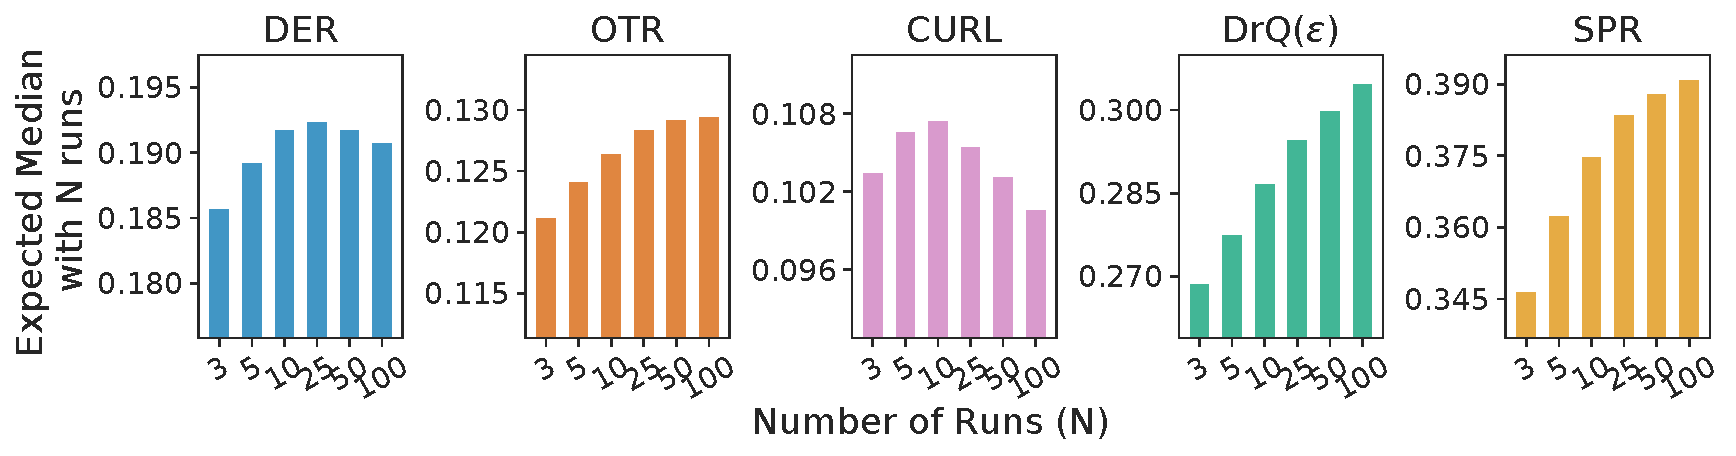
\includegraphics[width=0.95\linewidth]{new_figures/median_bias_all_algorithms_small.pdf}
    \vspace{-0.25cm}
    \caption{\textbf{Expected sample median} of task means. The expected score for $N$ runs is computed by repeatedly subsampling $N$ runs with replacement out of 100 runs for 100,000 times.}
    \label{fig:median_bias}
    \vspace{-0.1cm}
\end{wrapfigure}


% considerably? sizeably?
\textbf{Substantial bias in sample medians}. The sample median is a biased estimator of the true median: $\expected[\text{Median}({\bar X}_{1:M})] \neq  \text{Median}(\expected[X_{1:M}])$ in general. In the few-run regime, we find that this bias can dominate the comparison between algorithms, as evidenced in \figref{fig:median_bias}. For example, the score difference between sample medians with 5 and 100 runs for \spr~(+0.03 points) is about 36\% of its mean improvement over \drq$(\varepsilon)$~(+0.08 points). Adding to the issue, the magnitude and sign of this bias strongly depends on the algorithm being evaluated.




% \begin{wrapfigure}[24]{r}{0.41\linewidth}
%     \centering
%     \vspace{-0.55cm}
%     
\includegraphics[width=\linewidth]{figures/cis_iqm_vs_median_all_algos.pdf}
    % \vspace{-0.5cm}
%      \caption{\textbf{Left.} 95\% CIs for median normalized scores. \textbf{Right.} 95\% CIs for interquartile mean~(IQM) normalized scores~(\Secref{sec:better_aggregate}). As the number of runs increases, the uncertainty in results decreases, leading to smaller CIs. There is a substantial uncertainty in median scores even with 50 runs. IQM has much smaller CIs than median.
%     %  CIs are estimated by repeatedly subsampling K runs with replacement from 100 runs.
%      % We estimate these CIs by repeatedly sampling K runs out of 100 with replacement to approximate the median distribution and then calculate the interval between $2.5\%$ and $97.5\%$ percentiles of the median distribution.
%  }\label{fig:cis_upto_100}
%     \vspace{-0.7cm}
% \end{wrapfigure}

% Don't delete this!
% Uncertainty is sizeable, it does not ``go away'' in the few-run regime. For point estimates to be trustworthy, we need small uncertainty. Talk about statistical significance. Hypothesis test. Statistical validation of hypotheses.
% Variance of sample median-mean is not easy to write analytically.
% $m/n$ bootstrap confidence intervals. p-values.

% There is too much uncertainty, making it impossible to draw conclusions about effect size.

\textbf{Statistical concerns cannot be satisfactorily addressed with few runs.}
While claiming improvements with 3 or fewer runs may naturally raise eyebrows, folk wisdom in experimental RL suggests that 20 or 30 runs are enough.
By calculating 95\% confidence interval\footnote{Specifically, we use the $m/n$ bootstrap~\citep{bickel2012resampling} to calculate the interval between $[2.5^{th}, 97.5^{th}]$ percentiles of the distribution of sample medians ~(95\% CIs).} on sample medians for a varying number of runs (\figref{fig:variability_in_median}, right), we find that this number is closer to 50--100 runs in Atari 100k -- far too many to be computationally feasible for most research projects. 
% A typical approach to reason about the statistical validity of a hypothesis is to report
% \textbf{Detecting improvements between median scores require many runs}. We further find that the issue remains when computing $95\%$ CIs around the difference of sample medians (see Appendix for details).
% To show the uncertainty in sample medians, we compute their 95\% confidence intervals~(CIs) for different number of runs~(\figref{fig:cis_upto_100}). We estimate these CIs by
% calculating the interval between 2.5\% and 97.5\% percentiles
% of the distribution of sample median based on subsampled runs~(\eg \figref{fig:variability_in_median}). \figref{fig:cis_upto_100} shows that that $95\%$ CIs substantially overlap for DER, OTR and DrQ with 5 runs
% as well as for DrQ and SPR even when using as many as 50 runs. When CIs overlap for two random variables $X$ and $Y$ overlap, we estimate the $95\%$ CIs for $X - Y$ to account for uncertainty in their difference~(\figref{fig:diff_medians}). For example, when using 5 runs, the median score improvement from DrQ over DER is estimated to lie within $(0.01, 0.21)$ while that of SPR over DrQ lies within $(-0.09, 0.18)$. 
% Furthermore, while improvement from SPR over DER with $5$ to $25$ runs is not statistically significant, claiming ``no improvement'' would be misleading as evaluating more runs indeed shows that the improvement is significant.

% Don't delete this!
% Relative differences. How far we can be off from ``ground truth''. Detecting improvements directly. To make this point further ...
Consider a setting in which an algorithm is known to be better -- what is the reliability of median and IQM~(\Secref{sec:aggregate_metrics_robust}) for accurately assessing performance differences as the number of runs varies? Specifically, we consider two identical $N$-run experiments involving \spr, except that we artificially inflate one of the experiments' scores by a fixed fraction or \emph{lift} of $+\ell\%$ (\figref{fig:lift_spr}). In particular, $\ell = 0$ corresponds to running the same experiment twice but with different runs.
We find that statistically defensible improvements with median scores is only achieved for 25 runs~($\ell=25$) and 100 runs ($\ell=10$). With $\ell = 0$, even 100 runs are insufficient, with deviations of $20\%$ possible.
% shows that even with  $10\%$ and $25\%$ lifts, using lift in median scores to certainly claim an improvement requires at least 100 and 25 runs respectively. Similarly, even with 50 runs, the 95\% CI for observed median lift is estimated to be within $(10\%, 40\%)$ for $25\%$ lift. Furthermore, $0\%$ lift results show that even when comparing SPR with itself using two different sets of $10$ runs~(blue lines), it is possible to observe $40\%$ improvement or a $30\%$ degradation in median normalized scores.

% To compute how many runs are required for reliably reporting a certain improvement size, we consider an
% algorithm with an uniform lift of $\ell\%$ over SPR, that is, for runs with identical randomness, it obtains a $\ell\%$ higher normalized score than SPR. 

% \begin{wrapfigure}[14]{r}{0.42\linewidth}
%     \vspace{-0.45cm}
%     
\includegraphics[width=\linewidth]{figures/lift_median_vs_iqm_spr.pdf}
%     \vspace{-0.5cm}
%     \caption{ \textbf{Detecting score lifts}.
%     \textbf{Left}. $95\%$ CIs for observed lift with median scores, and \textbf{Right}. $95\%$ CIs for observed lift with IQM~(\Secref{sec:better_aggregate}) when comparing SPR with an algorithm that performs $\ell\%$ better. }
%     \label{fig:lift_spr}
% \vspace{-0.1cm}
% \end{wrapfigure}


% \begin{figure}[t]
%     \centering
%     \includegraphics[width=\linewidth]{figures/median_bias_all_algorithms.pdf}
%     \caption{\textbf{Bias in median scores}. Expected median human-normalized scores with varying number of runs. The expectation is computed by repeatedly subsampling a given number of runs with replacement out of 100 runs.}
%     \label{fig:median_bias}
%     \vspace{-0.4cm}
% \end{figure}


% \begin{figure}[t]
%     \begin{minipage}[t]{0.48\linewidth}
%         \vspace{0pt}
%         
\includegraphics[width=\linewidth]{figures/diff_median_cis.pdf}
%         \caption{ \textbf{Detecting score differences}.
%         \textbf{Left}. 95\% CIs for differences in median scores. \textbf{Right}. 95\% CIs for differences in IQM scores. Median requires many more runs than IQM for small uncertainty.}
%         \label{fig:diff_medians}
%     \end{minipage}~~
%     \begin{minipage}[t]{0.48\linewidth}
%         \vspace{0pt}
%         
\includegraphics[width=\linewidth]{figures/lift_median_vs_iqm_spr.pdf}
%         \caption{ \textbf{Detecting score lifts}.
%         \textbf{Left}. $95\%$ CIs for observed lift with median scores, and \textbf{Right}. $95\%$ CIs for observed lift with IQM~(\Secref{sec:better_aggregate}) as a function of number of runs when comparing SPR with an algorithm that performs $\ell\%$ better. }
%         \label{fig:lift_spr}
%     \end{minipage}
%     \vspace{-0.55cm}
% \end{figure}


